\chapter{In Depth: Manifold Learning\label{Ch46}}
While PCA is flexible, fast, and easily interpretable, it does
not perform so well when there are nonlinear relationships within the data.

\section{Multidimensional Scaling}
Given a distance matrix between points, it recovers a D-dimensional coordinate representation
of the data, this is exactly what the multidimensional scaling algorithm aims to do.

\subsection{MDS as Manifold Learning}

This is essentially the goal of a manifold learning estimator: given high-dimensional
embedded data, it seeks a low-dimensional representation of the data that preserves
certain relationships within the data. In the case of MDS, the quantity preserved is the
distance between every pair of points.

\begin{figure}
    \centering
    \begin{subfigure}[b]{.45\textwidth}
        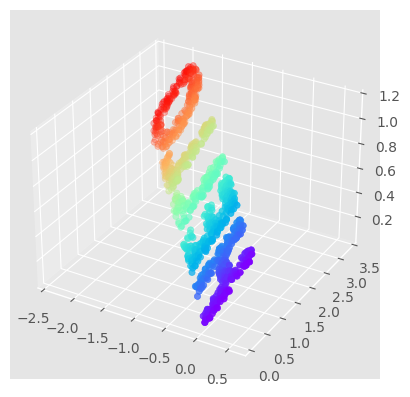
\includegraphics[width=\textwidth]{../Figures/fig46-5.png}
        \caption{Data embedded linearly into three dimensions}
    \end{subfigure}
    \hfill
    \begin{subfigure}[b]{.45\textwidth}
        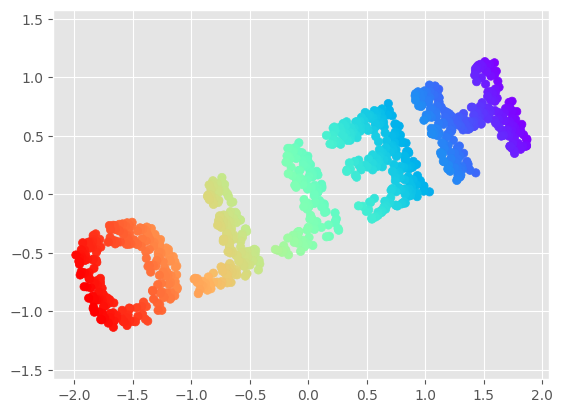
\includegraphics[width=\textwidth]{../Figures/fig46-6.png}
        \caption{The MDS embedding of the three-dimensional data recovers the input up to a rotation and reflection}
    \end{subfigure}
    \caption{MDS as Manifold Learning}
\end{figure}

\subsection{Nonlinear Embeddings: Where MDS Fails}
Where MDS breaks down is when the embedding is nonlinear—that is, when it goes beyond this simple set of operations.

\section{Nonlinear Manifolds: Locally Linear Embedding}
MDS tries to preserve distances between faraway points when constructing the embedding. But what if we instead modified the algorithm such that it
only preserves distances between nearby points? The resulting embedding would be
closer to what we want.

\begin{figure}
    \centering
    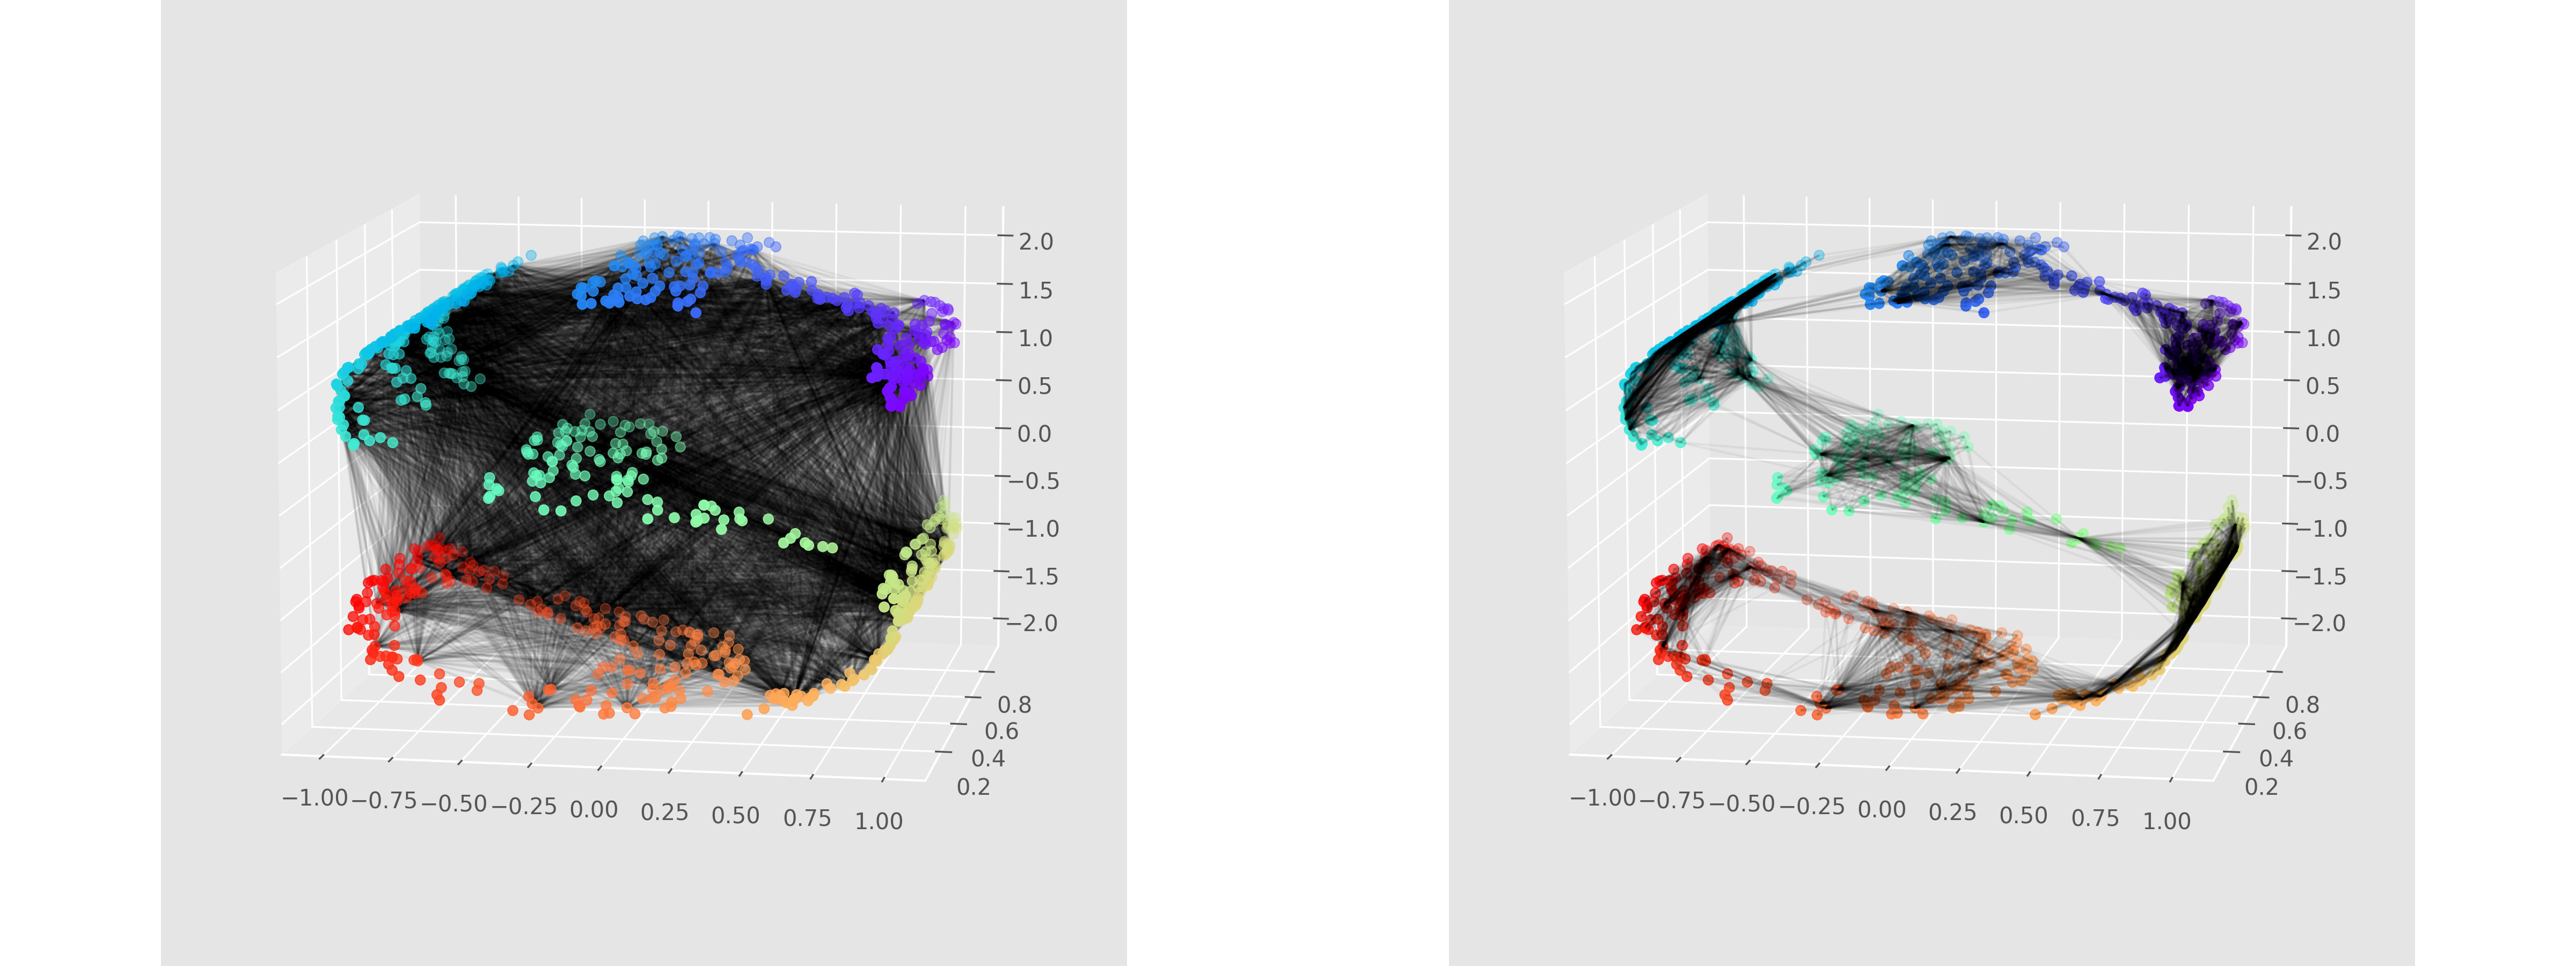
\includegraphics[width=\textwidth]{../Figures/fig46-7.png}
    \caption{Representation of linkages between points within MDS and LLE}
\end{figure}

\section{Some Thoughts on Manifold Methods}
In practice manifold learning techniques tend
to be finicky enough that they are rarely used for anything more than simple qualitative visualization of high-dimensional data.

The following are some of the particular challenges of manifold learning, which all
contrast poorly with PCA:
\begin{itemize}
    \item In manifold learning, there is no good framework for handling missing data. In contrast, there are straightforward iterative approaches for dealing with missing data in PCA.
    \item In manifold learning, the presence of noise in the data can “short-circuit” the manifold and drastically change the embedding. In contrast, PCA naturally filters noise from the most important components.
    \item The manifold embedding result is generally highly dependent on the number of neighbors chosen, and there is generally no solid quantitative way to choose an optimal number of neighbors. In contrast, PCA does not involve such a choice.
    \item In manifold learning, the globally optimal number of output dimensions is difficult to determine. In contrast, PCA lets you find the number of output dimensions based on the explained variance.
    \item In manifold learning, the meaning of the embedded dimensions is not always clear. In PCA, the principal components have a very clear meaning.
    \item In manifold learning, the computational expense of manifold methods scales as $O[N^2]$ or $O[N^3]$ . For PCA, there exist randomized approaches that are generally much faster (though see the \href{https://github.com/mmp2/megaman}{megaman package} for some more scalable implementations of manifold learning).
\end{itemize}

Based on my own experience, I would give the following recommendations:

\begin{itemize}
    \item For toy problems such as the S-curve we saw before, LLE and its variants (especially modified LLE) perform very well. This is implemented in sklearn.manifold.LocallyLinearEmbedding.
    \item For high-dimensional data from real-world sources, LLE often produces poor results, and Isomap seems to generally lead to more meaningful embeddings. This is implemented in sklearn.manifold.Isomap.
    \item For data that is highly clustered, t-distributed stochastic neighbor embedding (t-SNE) seems to work very well, though it can be very slow compared to other methods. This is implemented in sklearn.manifold.TSNE.
\end{itemize}